
\section{Library catalog data}
\begin{frame}{Theuerdank (Graz Sondersammlungen -- Rara 1 III 11723 )}
\footnotesize
    Pfintzing, Melchior, et al. Die geuerlicheiten und einsteils der geschichten des loblichen streytparen und hochberümten helds und Ritters herr Tewrdannckhs. 1517.

    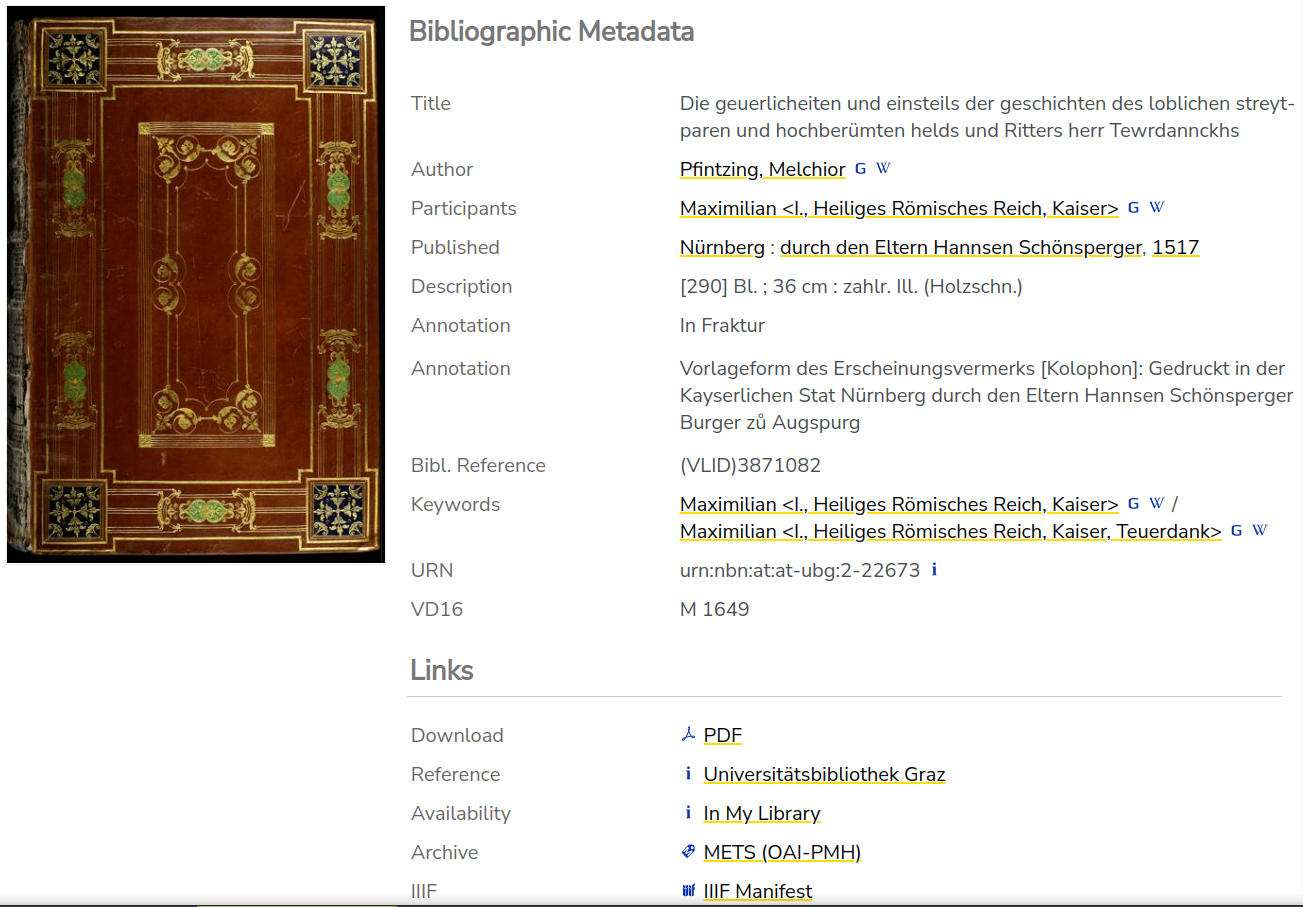
\includegraphics[width=0.95\textwidth]{img/theuerdank-biblio.png}
\end{frame}

%------------------------------------------------------------------------------
\begin{frame}[fragile,allowframebreaks]{MARC XML example}
    \footnotesize
    \href{https://lccn.loc.gov/2021667794/marcxml }{Library of Congress MARC XML for Theuerdank (simplified for demonstration purposes)}: \protect\url{https://www.loc.gov/item/2021667794}

    \begin{xmlcode}
<record xmlns="http://www.loc.gov/MARC21/slim" 
        xmlns:zs="http://docs.oasis-open.org/ns/search-ws/sruResponse">
    <leader>02892nam a22004093i 4500</leader>
    <controlfield tag="001">22061662</controlfield>

    <datafield ind1=" " ind2=" " tag="500">
      <subfield code="a">"BSB Shelfmark: Rar. 325 a"--Note extracted 
      from World Digital Library.</subfield>
    </datafield>
    
    <datafield ind1=" " ind2=" " tag="500">
      <subfield code="a">Original resource extent: 290 unnumbered 
      sheets : illustrations.</subfield>
    </datafield>
    [...]

</record>
\end{xmlcode}

    \begin{xmlcode}
<record xmlns="http://www.loc.gov/MARC21/slim" 
        xmlns:zs="http://docs.oasis-open.org/ns/search-ws/sruResponse">
        [...]
    
    <datafield ind1=" " ind2=" " tag="520">
      <subfield code="a">
      Among the many endeavors undertaken by the Holy Roman Emperor 
      Maximilian I (1459--1519) to further his legacy was his plan 
      of an epic retelling of his own life story in the form of 
      several works.       
      [...]
      Johann Schönsperger, a printer in Nuremberg, did the first, 
      very small print run in 1517, to be delivered to other princes 
      and sovereigns after the Emperor's death. 
      [...]
      Each of the 118 chapters is decorated by a xylograph 
      (wood engraving). The preparatory drawings for the xylographs 
      were created by the artists Leonhard Beck, 
      Hans Schäufelein, and Hans Burgkmair the Elder. The black-letter 
      type of the Theuerdank, designed by calligrapher Vinzenz Rockner, 
      was to become very influential for the development 
      of German typography.</subfield>
</datafield>

</record>
\end{xmlcode}

\end{frame}



